\chapter{Introduction}
\section{Plasma}
In this thesis we study the instability of plasma flow in magnetic mirror configuration. 
We start the thesis by introducing the concept of plasma.

Plasma is one of the four fundamental states of matter, along with solids, liquids, and gases. 
It is often referred to as the fourth state of matter. 
Plasma is an ionized gas that consists of highly energized particles, including positively charged ions and negatively charged electrons.

\begin{figure}[htbp]
    \centering
    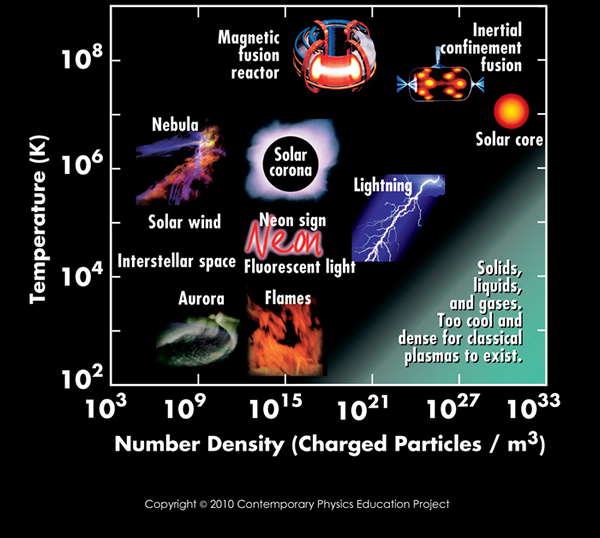
\includegraphics[width=0.7\textwidth]{img/introduction/plasma-properties}
    \caption{Characteristics of typical plasmas.}
    \label{fig:plasma-properties}
\end{figure}

In a plasma, the atoms or molecules have been stripped of their electrons, resulting in a collection of charged particles. 
This ionization process occurs when a gas is subjected to extremely high temperatures or strong electromagnetic fields, which supply sufficient energy to overcome the electrostatic forces that hold electrons in their orbits around atomic nuclei.

Plasma is known for its unique properties. 
It is an excellent conductor of electricity and is strongly influenced by electromagnetic fields. 
Plasma also emits light, and examples of natural plasma include stars, such as our Sun, and lightning. 
Artificially generated plasma can be found in fluorescent lights, plasma televisions, and certain types of industrial torches.

In addition to these applications, plasma has various scientific and technological uses. 
It is used in plasma physics research, nuclear fusion experiments, plasma cutting and welding, plasma medicine for treating diseases, and even in spacecraft propulsion systems.

Overall, plasma is an intriguing and versatile state of matter with significant implications in various fields of science, technology, and industry.

\subsection{Single Particle Motion Along Magnetic Field Line}
Since plasma consists of charged particles, its motion can is governed by Lorentz force. The equation of motion of a charged particle in magnetic field is given by
\[ m\dv{\mathbf{v}}{t} = q\mathbf{v\times B} \]
where $m$ is the mass of charged particle, and $q$ is the charge of particles.

Consider a magnetic field pointing in z-direction, $\mathbf{B}=B\mathbf{\hat{z}}$. Since the magnetic force is perpendicular to both $\mathbf{v}$ and $\mathbf{B}$, we can separate the equation of motion into two directions,
\[ 
q\mathbf{v_{\perp}\times B} = \frac{mv_{\perp}^2}{r}\mathbf{\hat{r}}, 
\quad
\mathbf{v}_{\parallel} = v_{\parallel} \mathbf{\hat{z}} \]
where $\mathbf{v}_{\perp}$ is the velocity perpendicular to the magnetic field, and $\mathbf{v}_{\parallel}$ is the velocity parallel to the magnetic field. In this way, we see that the charged particle gyrates about the magnetic field, doing helical motion along the magnetic field line. 

\begin{figure}[htbp]
	\centering
	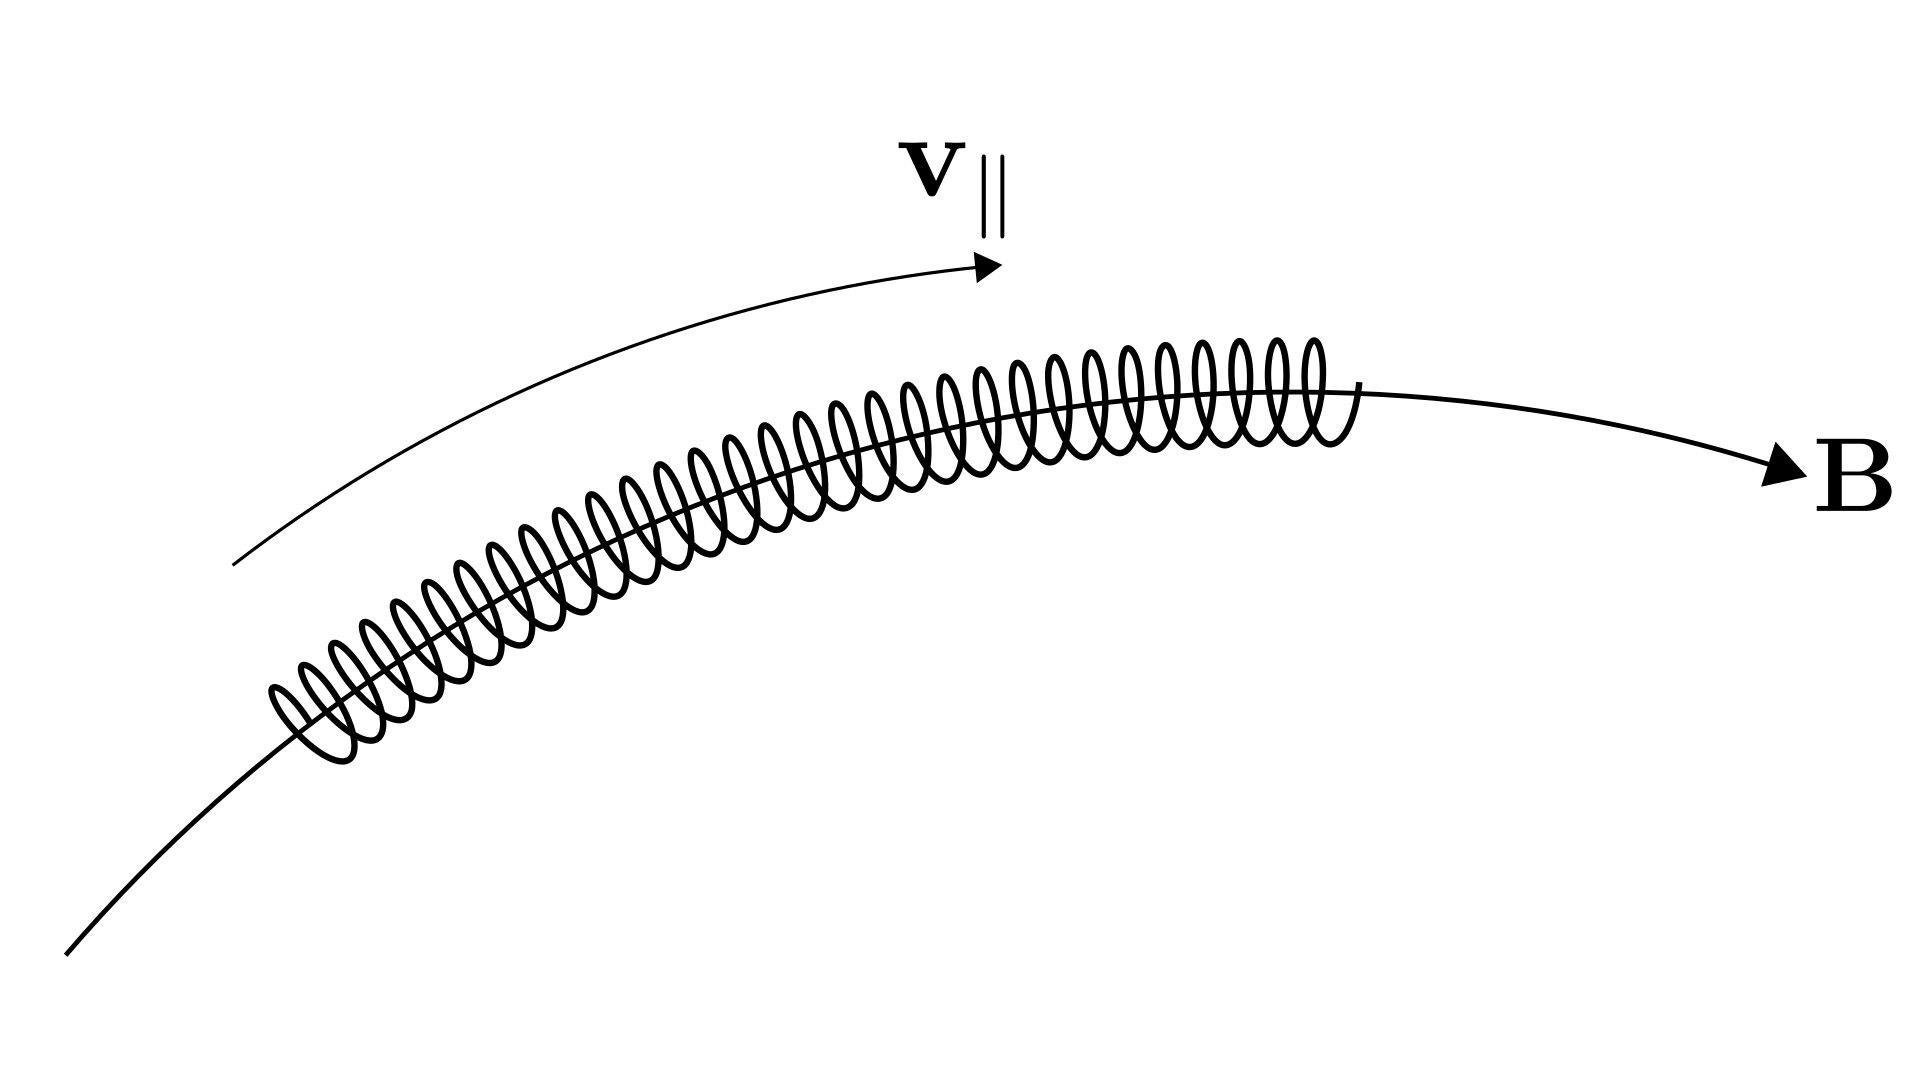
\includegraphics[width=0.7\linewidth]{img/governing-equations/gyrate-along-b-field}
	\caption{A charged particle gyrates about the magnetic field line. The velocity along the field line is $\mathbf{v}_{\parallel}$ and the gyrate frequency, radius is given by the radial equation, $q\mathbf{v_{\perp}\times B} = \mathbf{\hat{r}} mv_\perp^2/r$. Moreover, for static, nonuniform magnetic field, the charged particle will stay on the same of magnetic field line as it gyrates.}
	\label{fig:gyrate-along-b-field}
\end{figure}

\subsection{From Kinetic Theory to Fluid Description}
In kinetic theory, the charged particles in plasma obey a certain distribution function $f(\mathbf{x}, \mathbf{v}, t)$. This distribution function is affected by plasma temperature. Assuming there is only one species of particles in the plasma, the plasma temperature is just the sum of the kinetic energy of all particles. We expect at higher temperature, faster the particles will be.

Suppose a collisionless plasma is at equilibrium, then the particles can be characterized by Maxwell-Boltzmann distribution
\[ f_M(\mathbf{x}, \mathbf{v}, t) = \frac{1}{(\pi v_{th}^2)^{3/2}} \exp(-\left(\frac{v}{v_{th}}\right)^2) \]
where $v_{th} = \sqrt{2k_BT/m}$ is the thermal velocity.

The moments of the distribution function are suitable macroscopic properties of the plasma. For example, the plasma density and plasma momentum can be viewed as 
\[ n(\mathbf{x}, t) = \int_{\mathbb{R}^3} f(\mathbf{x}, \mathbf{v}, t) d^3\mathbf{v} \]
\[ n\mathbf{V}(\mathbf{x}, t) = \int_{\mathbb{R}^3} \mathbf{v}f(\mathbf{x}, \mathbf{v}, t) d^3\mathbf{v} \]
where $\mathbf{V}$ is the fluid velocity of the charged particle. It is the bulk velocity of the plasma. In magnetic nozzle, since the charged particles flow along the magnetic field line, it is intuitive to think of $\mathbf{V}$ as the plasma flow velocity along the magnetic field line.

In fusion device and space propulsion system, we want high plasma temperature to achieve good performance. Hence, we assume high plasma temperature in this thesis. In other words, the plasma is collisionless. 

The distribution function $f$ in a collisionless plasma satisfies the so-called collisionless Vlasov equation, $\dv*{t} f(\mathbf{x}, \mathbf{v}, t) = 0$. Expand it explicitly, it is
\begin{equation} \label{eq:vlasov}
	\pdv{f}{t} + \mathbf{v}\pdv{f}{\mathbf{x}} + \frac{q}{m}(\mathbf{E} + \mathbf{v}\times\mathbf{B})\pdv{f}{\mathbf{v}} = 0
\end{equation}
where $q(\mathbf{E} + \mathbf{v}\times\mathbf{B})$ is the Lorentz force experience by the species, the collision term $C(f)$ is dropped. Worth to mention that the electric field and magnetic field are generated by the configuration and the motion of the charged particles.

Integrate both sides with respect to volume element in velocity space, $d^3\mathbf{v}$, we get the conservation of density.
\[ \pdv{\rho}{t} + \div(\rho\mathbf{V}) = 0 \]

If we multiply $\mathbf{v}$ on both sides and integrate with respect to $d^3\mathbf{v}$, we get the conservation of momentum.
\[ \rho\pdv{\mathbf{V}}{t} + \mathbf{V}\cdot\grad{\mathbf{V}} = \frac{q}{m}(\mathbf{E+V\times B}) - \grad{p} \]
In the process we assume isotropic pressure, and no viscosity exists in the plasma.

As we can see the fluid description only depends on the macroscopic properties of plasma, such as the fluid velocity along the magnetic field line $\mathbf{V}$, density $\rho$, and pressure $p$ of the plasma. This simplifies the problem.

\section{Magnetic Nozzle}
In this thesis, we are going to deal with plasma flow in magnetic nozzle.
A magnetic nozzle is a device that uses a magnetic field to shape and control the flow of charged particles in a plasma propulsion system, see Fig.\ref{fig:magnetic-nozzle} . By employing magnetic mirrors, the magnetic nozzle can efficiently direct and accelerate the plasma particles, generating thrust for propulsion. The magnetic field in the nozzle helps collimate and focus the plasma exhaust, increasing its velocity and enhancing the performance of the propulsion system.

\begin{figure}[htbp]
	\centering
	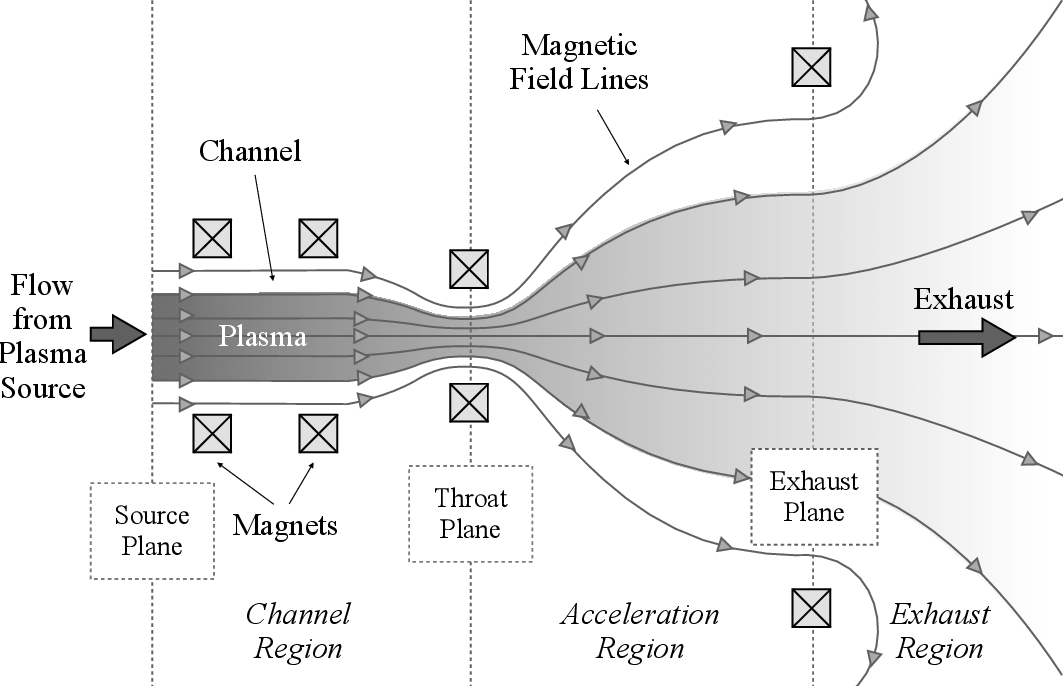
\includegraphics[width=0.7\linewidth]{img/introduction/magnetic-nozzle}
	\caption{Example of a magnetic nozzle configuration. In our models, we define the magnetic nozzle as the region downstream from the throat plane, which can be further divided into an acceleration region and exhaust region. The channel connects the plasma source (not shown) with the magnetic nozzle. \cite{little_performance_2015}}
	\label{fig:magnetic-nozzle}
\end{figure}

\subsection{Magnetic Field in Magnetic Nozzle} \label{sec:magnetic-field-in-nozzle}
This thesis will treat the flow in magnetic nozzle as a 1D motion. Hence, the magnetic field can be modeled as 
\[ B(z) = B_0 \left[1 + R\exp(-\left(\frac{x}{\delta}\right)^2)\right] \]
where $1+R$ is the magnetic mirror ratio, it is the ratio of the magnitude of magnetic field at the center of the nozzle to that at the end of the nozzle. Higher the magnetic mirror ratio, larger the difference between the magnitude of magnetic field at the center and at the end. On the other hand, $\delta$ determines the spread of the magnetic field. Larger the $\delta$, flatter the magnetic field. 

An example of magnetic field is shown in Fig.(\ref{fig:magnetic-field}).
\begin{figure}[H]
	\centering 
	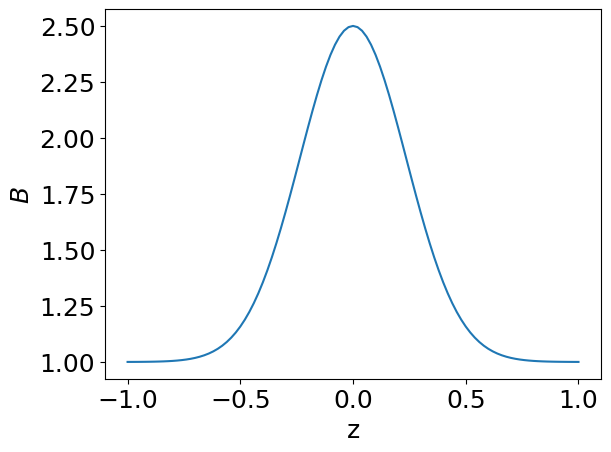
\includegraphics[width=0.7\linewidth]{img/governing-equations/magnetic-field}
	\caption{This is the magnetic field in nozzle with mirror ratio $1+R=B_{max}/B_{min}=2.5$, and the spread of magnetic field, $\delta=0.1/0.3=0.\bar{3}$. }
	\label{fig:magnetic-field}
\end{figure}


\subsection{Velocity Profile at Equilibrium}
Let $n_0$ and $v_0$ be the density and velocity at equilibrium, we know that $\pdv*{n_0}{t}=0$ and $\pdv*{v_0}{t}=0$ for the solution is stationary, in other words time independent. Therefore $n_0$ and $v_0$ satisfy the so-called equilibrium condition,
\begin{align*}
	&\pdv{z}(\frac{n_0v_0}{B}) = 0 \\
	&v_0\pdv{v_0}{z} = -c_s^2\frac{1}{n_0}\pdv{n_0}{z} 
\end{align*}

Let $M(z) = v_0(z)/c_s$ be the mach number (nondimensionalized velocity). The equations of motion become
\begin{align*}
	&B\pdv{z}(\frac{n_0M}{B}) = 0\\
	&M\pdv{M}{z} = -\frac{1}{n_0}\pdv{n_0}{z}
\end{align*}
Substitute $\frac{1}{n_0}\pdv*{n_0}{z}$ using first equation, the conservation of momentum becomes
\[ (M^2-1)\pdv{M}{z} = -\frac{M}{B}\pdv{B}{z} \]

Notice that there is a singularity at $M=1$, the sonic speed.

This is a separable equation, integrate it and use the conditions at midpoint $B(0)=B_m, M(0)=M_m$ we get
\[ M^2e^{-M^2} = \frac{B^2}{B_m^2}M_m^2e^{-M_m^2} \]
We can now express $M$ using the Lambert W function,
\[ M(z) = \left[ -W_k\left(-\frac{B(z)^2}{B_m^2}M_m^2e^{-M_m^2}\right) \right]^{1/2} \]
where the subscript $k$ of $W$ stands for branch of Lambert W function. When $k=0$, it is the subsonic branch; When $k=-1$, it is the supersonic branch. Below shows a few cases of the solution.
\begin{itemize}
	\item $M_m < 1, k=0$, subsonic velocity profile.
	\item $M_m = 1$, $k=0$ for $x<0$ and $k=-1$ for $x>0$, accelerating profile
	\item $M_m = 1$, $k=-1$ for $x<0$ and $k=0$ for $x>0$, decelerating profile
	\item $M_m > 1, k=-1$, supersonic velocity profile
\end{itemize}
 Fig.(\ref{fig:velocity-profiles}) shows some cases of the solution.
\begin{figure}[H]
	\centering
	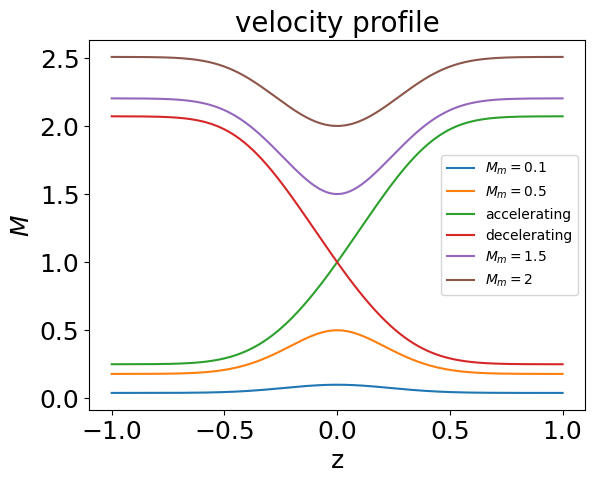
\includegraphics[width=0.7\linewidth]{img/governing-equations/velocity-profiles}
	\caption{The velocity profile in the magnetic nozzle is completely determined by $M_m$, the velocity at the midpoint, $z=0$. For the transonic velocity profiles, $M_m$ alone is not enough to determine the profile, we need to specify the branch of Lambert W function to determine whether it is accelerating or decelerating.}
	\label{fig:velocity-profiles}
\end{figure}

\subsection{Flow in Similar Configuration: Bondi-Parker Flow}
Bondi derived a steady-state solution for accretion flow which is governed by Bernoulli's equation in sperical symmetry around a point mass in 1952. Then Parker solved a similar problem but with outward wind in 1958. \cite{aikawa_stability_1979, bondi_spherically_1952,keto_stability_2020} The equilibrium velocity profiles in such configuration are shown in Fig.\ref{fig:BP-flow-velocity}.

\begin{figure}[htbp]
    \centering
    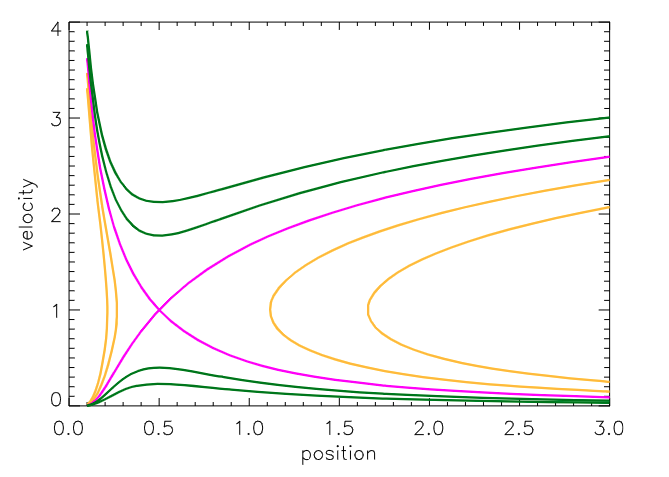
\includegraphics[width=0.7\textwidth]{img/introduction/steady-state-BP-flow}
    \caption{Representative trajectories of the steady-state BP flow in non-dimensional units. \cite{keto_stability_2020} The upward pink line represents a outward wind, it accelerates from subsonic to supersonic. The downward pink line represents an accretion flow, it accelerates towards the mass point. The green lines below the pink lines represent subsonic flows, and the green lines above represent supersonic flows. Orange lines are physically impossible scenarios.}
    \label{fig:BP-flow-velocity}
\end{figure}

Solar wind is an example of Bondi-Parker flow. The solar wind is a stream of charged particles, primarily electrons and protons, flowing outward from the Sun. 

In summary, the magnetic mirror configuration is a technique that uses magnetic fields to confine and control charged particles. It finds applications in plasma propulsion systems through the use of a magnetic nozzle. Moreover, the solar wind is another example of flows in magnetic mirror configuration. Its acceleration machanism is similar to that of magnetic nozzle. 

\section{Instability of Plasma Flow}
\subsection{Overview}
In this section, plasma instability will be introduced and from that we will discuss the importance of this research.

The instability of plasma flow refers to the tendency of a plasma system to deviate from a stable, equilibrium state and exhibit perturbations or fluctuations in its behavior. These instabilities can arise from various factors, such as the interaction of particles with electromagnetic fields, collective effects, or the presence of gradients in plasma parameters.

\begin{figure}[htbp]
	\centering
	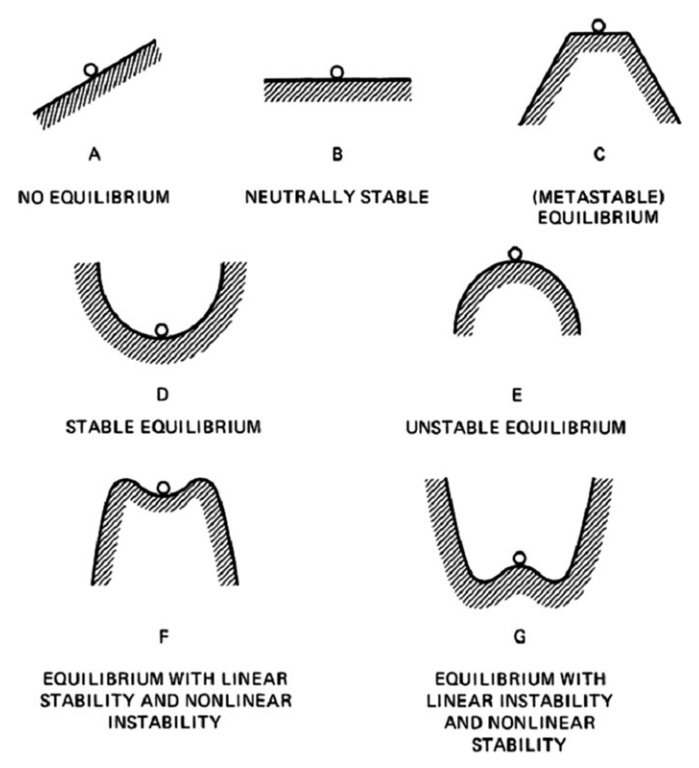
\includegraphics[width=0.7\linewidth]{img/introduction/stability-visualization}
	\caption{Mechanical analogy of various types of equilibrium. \cite{chen_introduction_2016}}
	\label{fig:stability-visualization}
\end{figure}

Understanding and studying plasma instabilities are crucial for several reasons:
\begin{enumerate}
    \item Energy Transport: Plasma instabilities can play a significant role in the transport of energy within a plasma system. They can enhance or hinder the transfer of energy between particles, affecting the overall efficiency and behavior of plasma devices. By studying these instabilities, scientists and engineers can gain insights into the mechanisms governing energy transport in plasmas and develop strategies to control and mitigate them.
    \item Plasma Confinement: In applications such as magnetic confinement fusion, achieving and maintaining a high degree of plasma confinement is essential for sustained fusion reactions. Instabilities can lead to the loss of plasma particles, reduction in confinement time, and decreased overall plasma performance. By understanding the nature of these instabilities, researchers can design improved confinement strategies and develop techniques to suppress or stabilize them.
    \item Plasma Heating: Instabilities can also influence the heating mechanisms in a plasma system. For example, in magnetic fusion devices, instabilities like the ion temperature gradient (ITG) or electron temperature gradient (ETG) instabilities can hinder efficient heating of the plasma. Understanding these instabilities helps in optimizing heating schemes and improving the overall heating efficiency of plasmas.
    \item Plasma Diagnostics: Instabilities can manifest as measurable fluctuations in plasma parameters such as density, temperature, and electromagnetic fields. By studying these fluctuations and their characteristics, scientists can employ diagnostic techniques to gain valuable information about the plasma state, identify the presence of instabilities, and assess the stability and health of plasma devices.
\end{enumerate}

\subsection{Illustration: Two-Stream Instability} \label{sec:two-stream-instability}
We take the famous two-stream instability as an illustration. Let the plasma be cold ($k_BT_e = k_BT_i = 0$), let there be no magnetic field ($B_0=0$). The linearized continuity equations are
\begin{align} 
	\pdv{n_{i1}}{t} + n_0\pdv{v_{i1}}{x} &= 0  \label{eq:two-stream-continuity1} \\
	\pdv{n_{e1}}{t} + n_0\pdv{v_{e1}}{x} + v0\pdv{n_{e1}}{x} &= 0 \label{eq:two-stream-continuity2}
\end{align}

And the linearized equations of motion are
\begin{align} 
	Mn_0\pdv{v_{i1}}{t} &= en_0E_1  \label{eq:two-stream-eom1} \\
	mn_0\left(\pdv{v_{e1}}{t} + v_0\pdv{v_{e1}}{x}\right) &= -en_0E_1 \label{eq:two-stream-eom2}
\end{align}
Here $v_0$ is the velocity of electron respect to the ions (the ion velocity at equilibrium is taken to be $v_{i0}=0$), $n_0$ is the equilibrium density of both ion and electron, $v_{i1}$ and $v_{e1}$ are perturbed velocity of ions and electrons, and $E_1$ is the perturbed electron field.

If we assume perturbed electric field takes the wave form
\[ E_1 = E\exp(i(kx-\omega t)) \]
Plug this perturbed electric field into Eq.(\ref{eq:two-stream-eom1}) and (\ref{eq:two-stream-eom2}), then we can solve for $v_{i1}$ and $v_{e1}$,
\begin{align*}
	v_{i1} &= \frac{ie}{M\omega} E \\
	v_{e1} &= -\frac{ie}{m}\frac{E}{\omega-kv_0}
\end{align*}

Using the perturbed velocities, the continuity equations Eq.(\ref{eq:two-stream-continuity1}) and (\ref{eq:two-stream-continuity2}) yields
\begin{align*}
	n_{i1} &= \frac{ien_0k}{M\omega^2} E \\
	n_{e1} &= \frac{iekn_0}{m(\omega-kv_0)^2}E
\end{align*}

Finally, plug them into the Poisson's equation
\[ \epsilon_0 \pdv{E_1}{x} = e(n_{i1}-n_{e1}) \]
We now have the dispersion relation
\[ 1 = \omega_p^2 \left[\frac{m/M}{\omega^2}+\frac{1}{(\omega-kv_0)^2}\right] \]

Solving this equation for $\omega$, there is chance we will get complex frequency,
\[ \omega = \omega_r + i\omega_i \]
where $\omega_r, \omega_i \in\mathbb{R}$. Then the perturbed electric field becomes
\[ E_1 = E\exp(i(kx-\omega_rt))\exp(\omega_it) \]

When $\omega_i < 0$, it is a damped wave. The amplitude of the wave will decay exponentially in time. When $\omega_i > 0$, the amplitude of wave grows exponentially in time and therefore unstable. Since the complex root comes with pair, as long as $\omega_i\neq 0$, one of the roots must correspond to an unstable wave. The following graph shows the two-stream instability in phase space.

\begin{figure}[H]
	\centering
	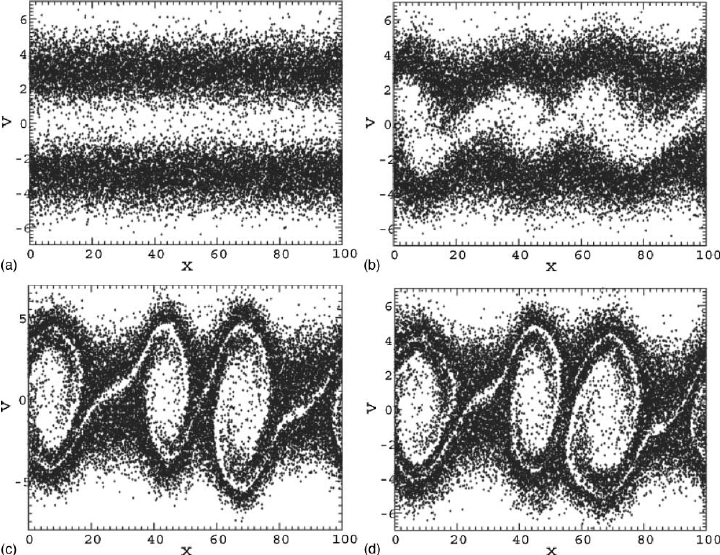
\includegraphics[width=0.7\linewidth]{img/introduction/two_stream_instability}
	\caption{Visualization of two-stream instability in the phase space. (a) Initially the ion and electron flow are in opposite direction. (b) The velocity of both flows start to oscillate. (c) Chaotic behavior occurs. (d) The chaotic behavior continues. \cite{ha_nonlinear_2011}}
	\label{fig:two-stream-instability}
\end{figure}


Overall, the study of plasma instabilities is crucial for advancing plasma physics research, optimizing plasma devices, and improving our ability to control and utilize plasmas effectively in various applications such as fusion energy, plasma propulsion, materials processing, and astrophysics.

\section{Goals of this Thesis}
The major goal of this thesis is to study the instability of plasma flow in magnetic mirror configuration with different boundary conditions.

Fluid model of plasma will be reviewed and linearized governing equations will be derived in chapter \ref{chap:governing-equations}. The problem will be then formulated as an eigenvalue problem.

In chapter \ref{chap:methodology}, spectral method and shooting method for solving eigenvalue problem will be introduced. 
In the section of spectral method, different discretizations of the operators, such as finite difference and spectral method will be discussed.
Moreover, spectral pollution and its filtering will as also be investigated.

Then in the next section, we will formulate the problem to the form suitable for applying shooting method. We will apply both shooting method and spectral method to the problem.
By comparing the results from two different methods, the credibility of the results are increased.

In chapter \ref{chap:numerical-experiments}, we ill use the method developed in chapter \ref{chap:methodology} to conduct numerical experiments. The goal is to extract the eigenvalues (frequency) of each oscillating mode. 

Conclusion will in chapter \ref{chap:conclusion}.